\part{SW 12}
\section{Lernziele (Leitfragen)}
\begin{itemize}
    \item Welche Adressen können in einem typischen TCP/IP Netzwerk gefälscht (spoof) werden? Was kann ein Angreifer erreichen, wenn eine solche Fälschung nicht erkannt oder verhindert wird?
    \item Geben Sie ein Beispiel von einem "`Man-in-the-middle"' Angriff
    \item Wie funktioniert einem "`Trust Exploitation"' Angriff?
    \item Geben Sie ein Beispiel für eine typische Softwareschwachstelle und eventuelle Folgen deren Nutzung (exploitation)
    \item Geben Sie ein Beispiel von einem "`Denial-of-Service"' Angriff
    \item Wieso sind "`Denial-of-Service"' Angriffe i.d.R. schwierig zu verhindern?
    \item Was ist "`Defense-in-depth"'?
    \item Wozu werden IDSs und IPSs verwendet? Wie unterschieden sie sich?
    \item Was Sind "`Data Loss Prevention Systems"'? Geben Sie ein Beispiel eines solchen Systems
    \item Geben Sie drei Beispiele von unsicheren Netzwerkprotokollen und deren entsprechenden sicheren Protokolle
    \item Wieso sind Backups wichtig? Was ist bei der Durchführung von Backups zu beachten (aus Sicherheits- und Betriebssicht)?
    \item Wieso ist Multifaktor Authentifizierung den Passwörtern zu bevorzugen?
    \item Was ist der Zweck einer Firewall?
    \item Wie funktioniert eine «First Generation (Packet Filter) Firewall»?
    \item Wie funktioniert eine «Second Generation (Stateful) Firewall»?
    \item Wie funktioniert eine moderne Firewall?
    \item Was ist ein «Proxy» und was ist sein Zweck?
    \item Was ist der Zweck einer Web Application Firewall (WAF)?
\end{itemize}

\section{Antworten}
\subsection*{Welche Adressen können in einem typischen TCP/IP Netzwerk gefälscht (spoof) werden? Was kann ein Angreifer erreichen, wenn eine solche Fälschung nicht erkannt oder verhindert wird?}\index{Spoofing}
Beispielsweise können MAC-Adressen, IP-Adressen wie Default-Gateway, DNS etc. gefälscht werden. Die Folge wäre ein DoS (Denial of Service).

\begin{figure}[H]
    \begin{center}
    \label{pic:Spoofing}
    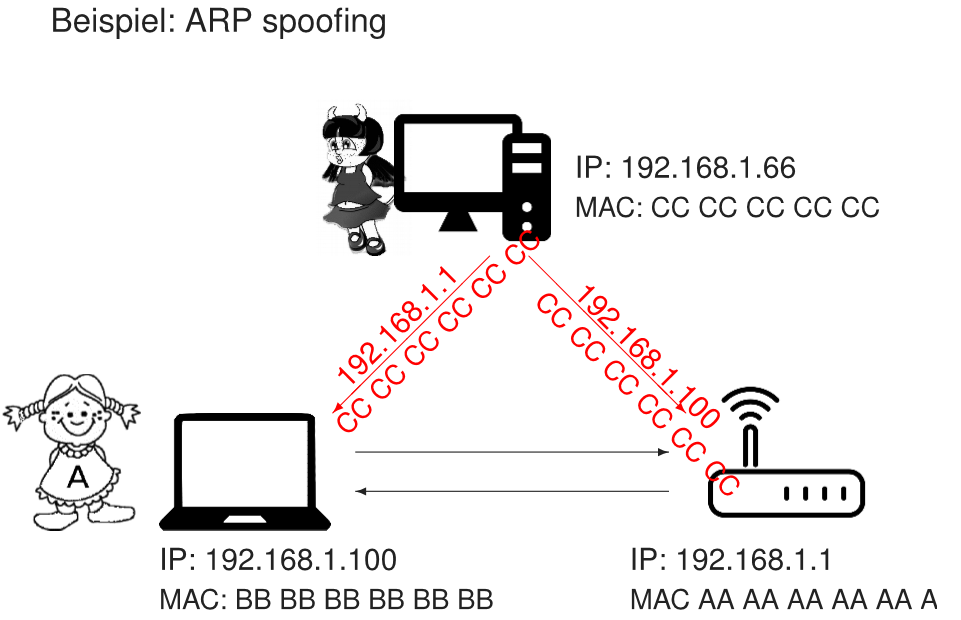
\includegraphics[width=\textwidth]{images/ARP_Spoofing.png}
    \caption{Beispiel ARP-Spoofing (Quelle: ISF Folien, Prof. Dr. Hänggi)}
    \end{center}
\end{figure}

\subsection*{Geben Sie ein Beispiel von einem "`Man-in-the-middle"' Angriff}\index{Man in the Middle}
Ein Angreifer stellt sich zwischen. Der Client (Victim) denkt, er ist mit dem Web Server im Kontakt jedoch ist der MITM ist dazwischen. Umgekehrt denkt der Web Server, dass der MITM der Client ist.
\begin{figure}[H]
    \begin{center}
    \label{pic:MITM}
    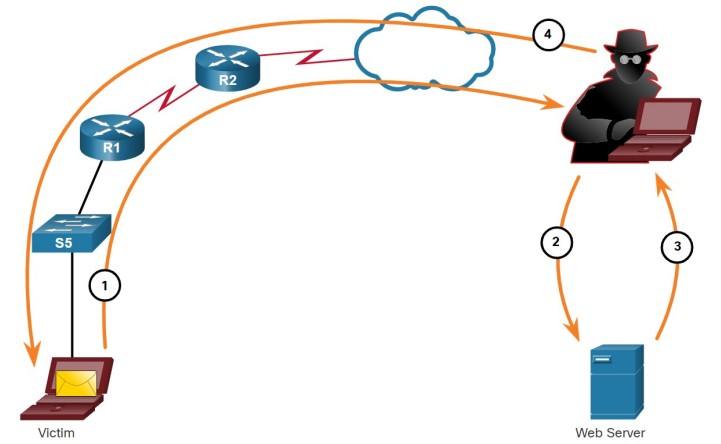
\includegraphics[width=\textwidth]{images/mitm.jpg}
    \caption{Man in the Middle (\textsuperscript{\textcopyright}Cisco)}
    \end{center}
\end{figure}

\subsection*{Wie funktioniert einem "`Trust Exploitation"' Angriff?}\index{Trust Exploitation}
Ein Angreifer nutzt das Vertrauen in Netzwerken aus. "`Befällt"' ein System und kommt durch Vertrauensnetz in das Netzwerk.

\begin{figure}[H]
    \begin{center}
    \label{pic:WOT}
    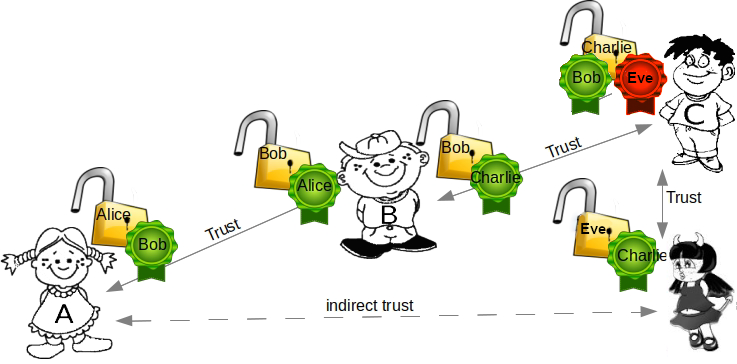
\includegraphics[width=\textwidth]{images/WOT.png}
    \caption{Web of Trust: Alice vertraut Eve indirekt (Quelle: ISF Folien, Prof. Dr. Hänggi, modifiziert)}
    \end{center}
\end{figure}

Eve konnte das Vertrauen von Charlie gewinnen, jedoch hat sie nichts gutes im Sinn.

\subsection*{Geben Sie ein Beispiel für eine typische Softwareschwachstelle und eventuelle Folgen deren Nutzung (exploitation)}\index{Vulnerability}\index{Schwachstelle}
RDP ist beispielsweise anfällig für Angriffe, wobei ein Angreifer die Kontrolle des Clients übernehmen kann.
\begin{figure}[H]
    \begin{center}
    \label{pic:RDPPenetration}
    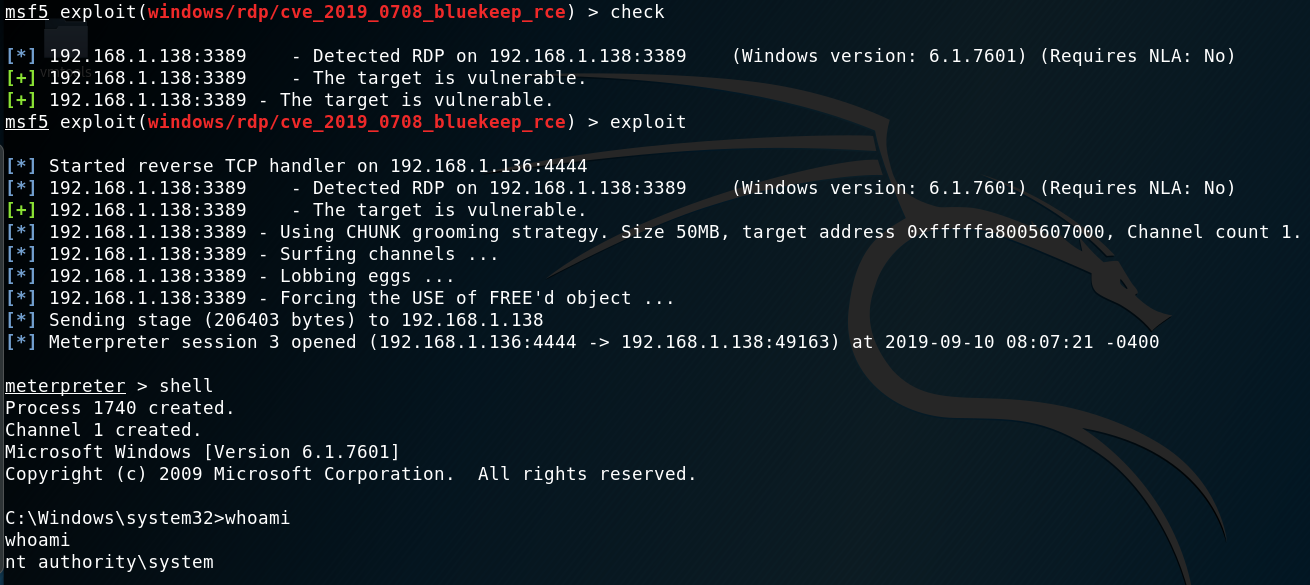
\includegraphics[width=\textwidth]{images/targets-set.png}
    \caption[Angriff auf RDP]{Angriff auf RDP\footnotemark}
    \end{center}
\end{figure}
\footnotetext{\url{https://pentest-tools.com/blog/wp-content/uploads/2019/09/targets-set.png}}

Früher konnte man auch, wenn man keine Administratorrechte hatte, über die Konsole mittels den Spooler-Service (Druckerwarteschlange) ein paar lustige Befehle eingeben, um Administratorrechte zu erlangen.\\
Nun, was heisst früher? Nach kleiner Internetrecherche ist das Problem wiedermal aktuell\footnote{\url{https://www.theregister.com/2021/06/30/windows_print_spool_vuln_rce/}}.

\subsection*{Geben Sie ein Beispiel von einem "`Denial-of-Service"' Angriff}\index{DoS - Denial of Service}
\begin{itemize}
    \item Angreifer sendet SYN requests an Webserver
    \item Webserver sendet SYN ACK reply an User und wartet auf SYN ACK
    \item Normaler User sendet aber auch SYN requests und der Server weiss nicht mehr, was er tun muss (DoS)
\end{itemize}

\begin{figure}[H]
    \begin{center}
        \label{pic:DoS}
        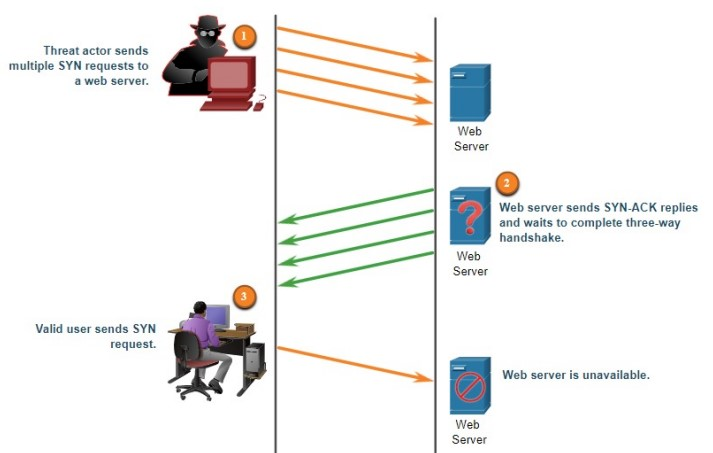
\includegraphics[width=\textwidth]{images/DoS.jpg}
        \caption{Beispiel Denial of Service (\textsuperscript{\textcopyright}Cisco)}
    \end{center}
\end{figure}

Es gibt Zwei Arten von DoS:
\begin{itemize}
    \item Buffer overflow Attacks
    \begin{itemize}
        \item sämtliche Ressourcen aufbrauchen
    \end{itemize}
    \item Flood Attacks
    \begin{itemize}
        \item den Server solange "`befeuern"', bis die Kapazität des Servers aufgebraucht ist
    \end{itemize}
\end{itemize}

\subsection*{Wieso sind "`Denial-of-Service"' Angriffe i.d.R. schwierig zu verhindern?}\index{DoS - Denial of Service}
Man weiss nicht, ob es ein Angreifer ist oder wirklicher Traffic

\subsection*{Was ist "`Defense-in-depth"'?}\index{Defense-in-depth}
Verschiedene Verteidigungsmechanismen auf verschiedenen Layern bereitstellen.

\subsection*{Wozu werden IDSs und IPSs verwendet? Wie unterschieden sie sich?}\index{IDS - Intrusion Detection System}\index{IPS - Intrusion Prevention System}
\begin{itemize}
    \item Intrusion Detection System: Ein Angriff wird erkannt und geblockt
    \item Intrusion Prevention System: Ein Angriff wird im Vornherein erkannt und unterbrochen.
\end{itemize}

\subsection*{Was Sind "`Data Loss Prevention Systems"'? Geben Sie ein Beispiel eines solchen Systems}\index{Data Loss Prevention Sysem}
Verhindern, dass sensitive Daten beispielsweise auf USB-Sticks kopiert werden, oder Emails keine sensitive Daten als Anhang haben.

\subsection*{Geben Sie drei Beispiele von unsicheren Netzwerkprotokollen und deren entsprechenden sicheren Protokolle}\index{Netzwerk!Sichere Protokolle}\index{FTP(S)}\index{HTTP(S)}\index{Telnet}\index{SSH}
FTP(S), HTTP(S), Telnet <-> SSH.

\subsection*{Wieso sind Backups wichtig? Was ist bei der Durchführung von Backups zu beachten (aus Sicherheits- und Betriebssicht)?}\index{Backups}
Im Falle eines Ausfalles, kann man die Daten aus dem Backup wieder zurückspielen, oder gar ganze Systeme aufsetzen (Clone). Backups müssen in regelmässigen Abständen gemacht werden (täglich bis wöchentlich). Die Backup-Drives müssen an einem anderen Standort gelagert werden, als dort wo der Server oder Client steht. Der Lagerort muss vor fremden Zugriff geschützt sein.

\subsection*{Wieso ist Multifaktor Authentifizierung den Passwörtern zu bevorzugen?}\index{MFA - Multifaktor Authentifizierung}
Mit MFA braucht es ein zusätzliches Authentifizierungsgerät (z.B. Smartphone: Google Authenticator, Microsoft Authenticator, SMS) neben dem Passwort. Dies erhöht die Sicherheit, falls das Passwort kompromittiert wurde, hat der Angreifer ohne den zusätzlichen MFA-Code keinen Zugriff auf das Benutzerkonto. Im Falle, dass das Smartphone nicht vorhanden ist (Akku leer), gibt es Backup-Codes, welche man bei der Erstellung der MFA bekommt. Diese müssen natürlich sicher verwahrt werden und vor fremden Zugriff geschützt werden.

\subsection*{Was ist der Zweck einer Firewall?}\index{Firewall}
\begin{itemize}
    \item Kontrollpunkt: Netzwerk-/ Datenverkehr erlauben oder verweigern
    \item Realisierung: Hard- und/oder Software
    \item Datenverkehr durch die Firewall muss autorisiert werden: Firewall-Rules
    \item Sie selbst muss gegen Angriffe möglichst resistent sein
\end{itemize}

\subsection*{Wie funktioniert eine «First Generation (Packet Filter) Firewall»?}\index{Firewall!1st Generation}
Vorteile:
\begin{itemize}
    \item Jedes Paket
    \begin{itemize}
        \item einzeln angeschaut
        \item in jede Richtung separat
        \item Paketinhalt nicht kontrolliert
    \end{itemize}
    \item In wenigen Fällen angewendet
    \item Kann mit modernen Routern realisiert werdenSehr schnell \& günstig
\end{itemize}
Nachteile:
\begin{itemize}
    \item Schwierig zu konfigurieren
    \item Probleme mit gewissen Protokollen wie FTP
    \begin{itemize}
        \item Ankommende Verbindung für FTP Data
    \end{itemize}
    \item Keine Zusammenhänge zu vorhergehenden Paketen
    \item Probleme mit Protokollen mit dynamischen Port-Nummern
    \item Paket-Inhalt (Daten) wird \textbf{nicht} kontrolliert!
\end{itemize}

\subsection*{Wie funktioniert eine «Second Generation (Stateful) Firewall»?}\index{Firewall!2nd Generation}
\begin{itemize}
    \item Paket-Filter mit Intelligenz
    \item Zusammenhänge zwischen Paketen werden berücksichtigt
    \item Antwort auf ein vorher ausgehendes Paket wird wieder reingelassen
    \item Paket-Inhalt (Daten) nicht kontrolliert
\end{itemize}

\subsection*{Wie funktioniert eine moderne Firewall?}\index{Firewall!Modern}
\begin{itemize}
    \item System: Software und ev. Hardware
    \item Kann (auch) ausgefeilte Angriffe erkennen und blockieren
    \item Fassen drei Schlüsselfunktionen zusammen:
    \begin{itemize}
        \item Techniken von professionellen (stateful) Firewalls
        \item Intrusion Detection \& Prevention Systems (IDS \& IPS)
        \item Applikations-Kontrolle (mittels Deep-Packet-Inspection)
    \end{itemize}
    \item Evtl. externe (freie und kostenpflichtige) Quellen (feeds) mit weiteren Informationen integriert
    \begin{itemize}
        \item Somit könnten z.B. bei einer bekannt gewordenen Phishing-Attacke automatisch solche Sites direkt auf der Firewall gesperrt werden
    \end{itemize}
\end{itemize}

\subsection*{Was ist ein «Proxy» und was ist sein Zweck?}\index{Proxy}
Vorteile:
\begin{itemize}
    \item Einfacher zu konfigurieren
    \item Keine vertieften TCP/IP Kenntnisse erforderlich
    \item Relativ sicher im Vergleich zu Packet Filter
\end{itemize}
Nachteile:
\begin{itemize}
    \item Relativ langsam im Vergleich zum Paket-Filter
    \item Falls neue oder nicht unterstützte Protokolle verwendet werden, sollen, muss eine neue Firewall-Software entwickelt werden
    \item Ressourcenintensiv
\end{itemize}

\subsection*{Was ist der Zweck einer Web Application Firewall (WAF)?}\index{WAF - Web Application Firewall}
\begin{itemize}
    \item Schutz eines oder mehrerer Web-Server
    \item Zusätzlich zur "`normalen"' Firewall (nicht als Ersatz)
    \item Schutz gegen SQL-Injection, XSS etc. (z.B. OWASP Top 10)
    \item Evtl. Validierung von Cookies, Session State, User etc.
    \item Proaktiver Schutz gegen neue (ev. noch nicht entdeckte) Sicherheitslücken
    \item Know-How Transfer Software-Entwickler $\rightarrow$ Firewall Administrator
\end{itemize}

Zu den Funktionalitäten einer WAF gehören
\begin{itemize}
    \item Terminierung der SSL-Verbindung
    \item Protokoll-Einschränkungen
    \item Load Balancing
    \item DoS-Verhinderung
    \item Session-Management (Cookie-Store, Timeouts)
    \item Filter gegen SQL-, HTML- und Code-Injection, XSS (Cross-Site Scripting)
    \item URL-Verschlüsselung
    \item Fehlerseiten umschreiben
    \item Request- und Response-Header setzen, entfernen, blockieren
    \item CSRF-Token (Cross-Site Request Forgery) einfügen
    \item `Dynamic Value Endorsement'
    \item Logging und Monitoring
\end{itemize}
